\documentclass[10pt]{article}
\usepackage[letterpaper,margin=0.82in]{geometry}
\usepackage{amsmath,amssymb,booktabs,array}
\usepackage{tikz}
\usepackage{pgfplots}
\pgfplotsset{compat=1.18}
\usepackage[colorlinks=true,allcolors=blue]{hyperref}
\usepackage{microtype}
\setlength{\parindent}{1em}
\setlength{\parskip}{0.25em}
\setlength{\abovedisplayskip}{7pt}
\setlength{\belowdisplayskip}{7pt}
\newcommand{\E}{\mathbb{E}}
\newcommand{\Sterm}{S}
\newcommand{\Tterm}{T}
\title{Trait Growth against the Selection Differential: A Lineage Audit of Bounded Mutation}
\author{}
\date{October 27, 2026 \quad---\quad Research draft}
\begin{document}
\maketitle
\vspace{-1.7em}
\begin{abstract}
A bounded heritable trait can increase from an absent founder while its realized selection differential is negative. We audit this distinction in a spatial artificial-life system using the exact clipped-Gaussian mutation drift and a standard Price decomposition. Forty-eight runs compare a neutral trait, a cost-only trait, and thermal sensing. The prospectively specified prediction of cost-only growth to at least $.02$ while cumulative selection is at most $-.02$ fails: only $1/16$ seeds pass, against a required $12/16$. Nevertheless, all cost-only populations retain a small positive trait mean, with mean transmission $+.3477$ opposing a selection differential of $-.3318$. Their final living mean is $.0159$, whereas recent newborns average $.0296$. Replacing the endpoint after seeing the data would change the size check from $1/16$ to $16/16$; we do not make that substitution. This negative test and descriptive sensitivity analysis contribute a reproducible audit of trait-growth interpretations, grounded in established mutation-bias and Price-equation theory.
\end{abstract}

\section{The question}
Artificial-life experiments often ask whether an initially absent, costly capability can evolve. A common implementation represents its intensity by a real number $h\in[0,1]$, initializes $h=0$, and perturbs the inherited value at reproduction. If the population subsequently has $\bar h>0$, innovation has occurred. Whether differential survival and reproduction favored increasing $h$ is a separate question.

This distinction matters in \emph{active-loop}, a research platform that studies embodied agents with energy budgets, resource competition, inherited traits, and learned resource maps. Earlier sensing experiments tracked living and newborn trait averages. Newborn measurements avoid conditioning solely on which offspring survive to a later census, but they still combine which parents reproduce with how mutation changes their offspring. The latest laboratory audit also emphasizes that a recorded outcome must be distinguished from the stronger interpretation attached to it. These observations motivate an instrument-level question: \emph{can the trait grow while its realized selection differential points downward?}

Boundary handling is already known to influence evolutionary algorithms and to create structural bias unrelated to objective values~\cite{caraffini,boks}. The separation between selection and transmission is the standard Price equation~\cite{price,frank}; its empirical use in digital life, including comparisons with neutral markers, also predates this study~\cite{mirmomeni}. We therefore claim neither a new theorem about selection nor the first use of lineage accounting in artificial life.

Our contribution is a reproducible audit of a particular costed-capability experiment: an analytic benchmark for its actual mutation rule, an observation-only implementation for its overlapping population, and a fresh-cohort test of an explicit sign-reversal prediction. The audit does not replace a fitness assay or an invasion experiment. It identifies which component of the measured evolutionary change actually carries the increase.

\newpage
\section{Boundary drift and exact lineage accounting}
\subsection{The mutation operator is not mean-preserving near a boundary}
For $L\le U$ and $\sigma>0$, let an offspring value be
\begin{equation}
 h'=\min\{U,\max\{L,h+\sigma Z\}\},\qquad Z\sim\mathcal N(0,1).
\end{equation}
Write $a=(L-h)/\sigma$, $b=(U-h)/\sigma$, with standard normal density $\phi$ and distribution function $\Phi$. Splitting the expectation at the two clipping boundaries gives
\begin{equation}\label{eq:drift}
 d_\sigma(h):=\E[h'-h\mid h]
 =\sigma[\phi(a)-\phi(b)]+(L-h)\Phi(a)+(U-h)[1-\Phi(b)].
\end{equation}
The interior contribution is $\sigma\int_a^b z\phi(z)\,dz=\sigma[\phi(a)-\phi(b)]$; the other terms are the two boundary atoms. For $L=0$, $U=1$, and $\sigma=.05$, the expected increment at zero is $0.0199471$ (the upper-bound correction is negligible). At $h=.05$ it is $0.00416577$; at $h=.1$ it is $0.000424535$; at the midpoint it is zero. Thus a nominally centered perturbation has a directional transmission effect precisely where a new capability starts.

\paragraph{Boundary innovation cannot be mean-unbiased.}
More generally, let an offspring trait $X\in[0,U]$ descend from $h=0$. If $\Pr(X>0)>0$, then $\E[X]>0$: a nonnegative random variable has zero expectation only if it is zero almost surely. Consequently, reflection, rejection, or another bounded mutation rule cannot simultaneously preserve the mean at zero and permit positive innovation there. This elementary observation argues for measuring transmission, rather than searching for a boundary convention that removes this distinction.

\subsection{A census-to-census Price ledger}
At step $t$, let $P_t$ contain $N_t>0$ individuals with traits $h_i$, and assume $N_{t+1}>0$. For each $j\in P_{t+1}$, let $a(j)\in P_t$ be its ancestor: itself if it survived, or its recorded parent if it was born. Define
\begin{align}
 S_t&=\frac{1}{N_{t+1}}\sum_{j\in P_{t+1}} h_{a(j)}-\bar h_t,\label{eq:selection}\\
 T_t&=\frac{1}{N_{t+1}}\sum_{j\in P_{t+1}}(h_j-h_{a(j)}).\label{eq:transmission}
\end{align}
Adding and subtracting the ancestral mean gives the exact identity
\begin{equation}\label{eq:price}
 \bar h_{t+1}-\bar h_t=S_t+T_t,
 \qquad \bar h_H-\bar h_0=\sum_{t=0}^{H-1}S_t+\sum_{t=0}^{H-1}T_t.
\end{equation}
With $w_i$ the number of after-census descendants, including self-survival, $S_t=\operatorname{Cov}_{P_t}(w_i,h_i)/\bar w$. This is a \emph{realized selection differential}, not an identified causal effect of $h$. Drift, age structure, spatial assortment, and linkage to other traits can contribute~\cite{okasha}. Even the neutral marker need not have $S_t=0$.

Here newborns neither act nor die before the next step, and inherited $h$ does not change within a survivor. Consequently, only newborns contribute to $T_t$. Their actual parent values also define the conditional kernel benchmark $B_t=N_{t+1}^{-1}\sum_{j\,\mathrm{newborn}}d_\sigma(h_{a(j)})$. We report $T_t-B_t$ descriptively, without claiming a calibrated martingale test. Extinction leaves the next mean undefined and must be reported, not replaced by a successful zero-change step.

\newpage
\section{Prospectively specified experiment}
\paragraph{Substrate.}
We reuse the zero-founder thermosense configuration from the platform's Experiment 198, without modifying the ecology engine or mutation operator. Twelve founders inhabit a $12\times12$ resource grid. Creatures spend energy, forage using a learned resource map and a provided movement policy, reproduce subject to energy constraints, and die. Multiple other traits mutate alongside $h$; this is not a single-locus causal intervention. Mutation adds a Gaussian with standard deviation $.05$ times each trait's allowed range, then clips. The focal range is $[0,1]$, so its standard deviation is $.05$.

The three conditions below all start at $h=0$. An organ is expressed when $h$ strictly exceeds its activation threshold. Expressed upkeep is $.02+e h$, where inherited inefficiency $e\in[.2,1]$. Below the threshold, upkeep is zero. The thermal condition also provides a temperature field, a drifting comfort target, and the original sensing policy. The neutral condition disables temperature and sets the activation threshold to $1$, leaving $h$ heritable but with no direct functional use or upkeep.

\begin{center}
\begin{tabular}{lccc}
\toprule
Condition & Temperature & Activation threshold & Focal trait role\\
\midrule
Neutral & Off & $1.00$ & No direct function or cost\\
Cost-only & Off & $0.05$ & Upkeep, no sensing benefit\\
Thermal & On & $0.05$ & Upkeep and thermal sensing\\
\bottomrule
\end{tabular}
\end{center}

\paragraph{Fixed design and decision rule.}
Before simulation, the design was committed as \texttt{32f2c19}. Confirmation uses seeds $9500,\ldots,9515$, a horizon of $H=3000$ steps, and an emergency population ceiling of $5000$. Excluded seed $9499$ is reserved for timing and instrument checks. No equilibrium or long-term stationarity is assumed. The primary prediction requires at least $12/16$ cost-only runs to satisfy \emph{all three} conditions: completion without extinction or explosion, final living mean $\bar h_H\ge .02$, and cumulative differential $\sum_tS_t\le-.02$. A second conjunct requires neutral final living mean at least $.02$ in at least $12/16$ runs. Thermal outcomes are descriptive; no directional thermal comparison is preregistered.

Failure of either scientific conjunct makes the experiment negative. Extinct and interrupted runs remain in the denominator. Missing ancestry or a Price-identity error greater than $10^{-10}$ is an instrument failure. Thresholds are decision rules for this case study, not universal definitions of adaptation. We also report the mean trait of all births in the final $500$ steps; this is a separate diagnostic and does not replace the living-census endpoint.

\paragraph{Implementation and verification.}
The observer reads the before/after living populations and parent IDs; it draws no random numbers and changes no organism. Newborns are added only after existing creatures act, making the ancestry map in Eqs.~\eqref{eq:selection}--\eqref{eq:transmission} valid. A parent may die after reproducing and still contributes descendants. The ledger takes $O(N_t+N_{t+1})$ work per step, rather than rescanning all historical births. Hand-calculated pedigree tests, missing-parent checks, analytic mutation checks, and observed-versus-unobserved event hashes guard the instrument. Independent seed/condition runs execute in parallel after a runtime and memory preflight.

\newpage
\section{Results}
\paragraph{The primary prediction fails.}
All $48$ runs completed $3000$ steps without extinction or explosion. Every cost-only seed had $\sum_tS_t\le-.02$, but only seed $9512$ reached $\bar h_H\ge .02$. The cost-only conjunction is therefore $1/16$, below the required $12/16$. The neutral conjunct passes $16/16$. The combined prespecified verdict is \textbf{negative}; the small-floor observations below do not rescue it.

\begin{center}\small
\begin{tabular}{lrrrrr}
\toprule
Condition & Living $\bar h_H$ & Newborn mean & $\sum S$ & $\sum T$ & Final $N$\\
\midrule
Neutral & .086955 & .088510 & $-.131253$ & .218208 & 520.1\\
Cost-only & .015910 & .029583 & $-.331808$ & .347717 & 453.8\\
Thermal & .040868 & .043914 & $-.374624$ & .415491 & 81.9\\
\bottomrule
\end{tabular}
\end{center}
\noindent Table 1: Arithmetic means over sixteen independent seeds per condition. Newborns are all births in steps $2500\le t<3000$, including offspring that later died. Cumulative terms are signed trait changes; their sum equals the living endpoint because founders have $h=0$. They are not percentages or causal effect estimates.

\begin{figure}[h!]
\centering
% BEGIN GENERATED SCATTER
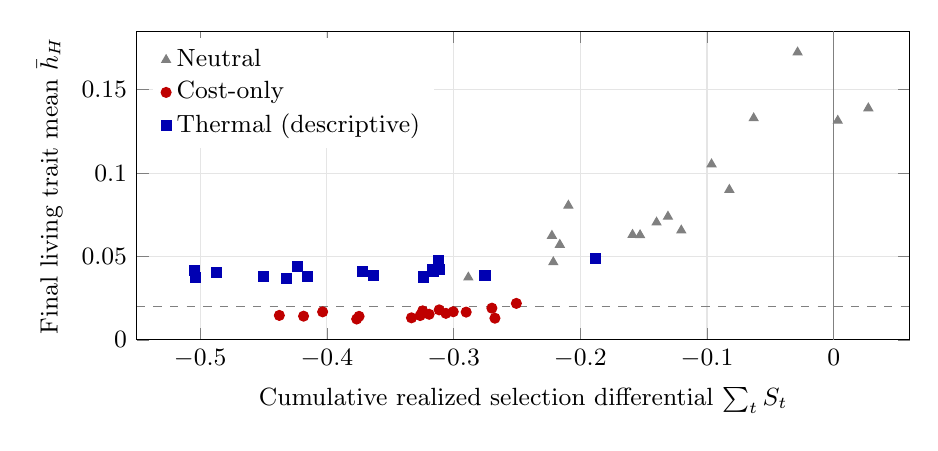
\begin{tikzpicture}
\begin{axis}[width=0.94\linewidth,height=5.5cm,
xmin=-.55,xmax=.06,ymin=0,ymax=.185,grid=major,grid style={gray!20},
xlabel={Cumulative realized selection differential $\sum_t S_t$},
ylabel={Final living trait mean $\bar h_H$},
scaled ticks=false,xtick={-.5,-.4,-.3,-.2,-.1,0},ytick={0,.05,.10,.15},
tick label style={font=\small,/pgf/number format/fixed,/pgf/number format/precision=2},label style={font=\small},
legend style={at={(0.02,0.98)},anchor=north west,font=\small,draw=none,fill=white},
legend cell align=left]
\addplot[gray,dashed,forget plot] coordinates {(-.55,.02) (.06,.02)};
\addplot[gray,thin,forget plot] coordinates {(0,0) (0,.185)};
\addplot[only marks,mark=triangle*,mark size=1.8pt,color=gray] coordinates {(-0.139818022077,0.070429589482) (0.003197024208,0.131463857067) (-0.028512073245,0.172426952121) (-0.152813675111,0.062846378957) (-0.222381500193,0.062479295953) (-0.209400339049,0.080557729662) (-0.096420667349,0.105335385432) (-0.082363983611,0.090031242368) (-0.120299457667,0.065668955443) (-0.221306800129,0.046614103389) (-0.158768564303,0.063038979682) (0.027318923874,0.138918112775) (-0.130812224143,0.073972515342) (-0.216146481562,0.057087908305) (-0.288353200405,0.037468018698) (-0.063161062301,0.132939407193)};
\addlegendentry{Neutral}
\addplot[only marks,mark=*,mark size=1.8pt,color=red!75!black] coordinates {(-0.437517913729,0.014690690714) (-0.290063122357,0.016678620873) (-0.324399220227,0.017421828001) (-0.267367204011,0.013026695039) (-0.333224063419,0.013241377855) (-0.311352049578,0.018020468349) (-0.403344729879,0.016837919428) (-0.326387180183,0.014604438182) (-0.376460943344,0.012525790739) (-0.319288908514,0.015373469051) (-0.418390635937,0.014242389554) (-0.269757896036,0.019037105658) (-0.250451154738,0.021894541789) (-0.306062293829,0.015930432347) (-0.300254467690,0.016890751352) (-0.374598367933,0.014137578112)};
\addlegendentry{Cost-only}
\addplot[only marks,mark=square*,mark size=1.8pt,color=blue!70!black] coordinates {(-0.316861419585,0.041986337362) (-0.449885653400,0.038041966359) (-0.275188336394,0.038861011146) (-0.432187789893,0.036802791130) (-0.312091856241,0.047502588176) (-0.323955178205,0.037707517642) (-0.415315043130,0.037823387289) (-0.503852087537,0.037266009481) (-0.315689088942,0.041092001237) (-0.188213936606,0.048786990046) (-0.311087230740,0.042346944600) (-0.504197931540,0.041538804381) (-0.423267591115,0.044054932914) (-0.487050076212,0.040681099994) (-0.371597304798,0.040885629219) (-0.363535771005,0.038507721260)};
\addlegendentry{Thermal (descriptive)}
\end{axis}
\end{tikzpicture}
% END GENERATED SCATTER
\caption{All forty-eight seeds: the living trait endpoint against its cumulative realized selection differential. The dashed line is the fixed $.02$ size bar. Fifteen cost-only points lie below it despite positive trait values. Thermal results are descriptive, not a replacement confirmatory test.}
\end{figure}

\paragraph{Endpoint sensitivity is substantial, but post hoc.}
Cost-only living means span $.012526$--$.021895$; newborn means span $.025965$--$.032589$. Substituting newborn mean for the registered living endpoint would make all $16$ size checks pass. That is an exploratory sensitivity result, not a revised verdict. A weaker rule that merely equates positive trait growth with adaptation would also label every cost-only run, despite a negative differential in all sixteen.

\paragraph{A common mutation rule does not cancel its accumulated contribution.}
Descriptively, thermal-minus-cost living mean is $+.024958$, while the corresponding difference in $\sum S$ is $-.042816$ and in $\sum T$ is $+.067774$. Thus the positive endpoint contrast does not equal a positive contrast in the selection differential. Different demography and parental distributions enter both terms. These are accounting contrasts, not causal mediation estimates.

\paragraph{Instrument checks.}
Across $144{,}000$ transitions, maximum identity error was $5.04\times10^{-17}$ (rounded upward); maximum telescoping error was $1.03\times10^{-15}$. Mean $\sum(T-B)$ was $.000906$, $.006053$, and $.017994$ for neutral, cost-only, and thermal conditions. These stochastic discrepancies are reported without an equivalence claim. The observer preserved all three excluded-pilot event hashes.

\newpage
\section{Implications and limits}
The relevant question is not whether the mutation operator is allowed to introduce a capability: introduction is its purpose. The problem is interpreting an increase without separating transmission from differential persistence. Clipping supplies a positive input near zero, and a cost can remove some of that input while leaving a nonzero population mean. This is a mutation--selection process, not automatically evidence that greater capability is favored.

A newborn-only endpoint does not solve the attribution problem. Algebraically, the newborn mean minus the all-parent mean equals the difference between the reproductive-parent mean and the all-parent mean, plus mean child-minus-parent transmission. It still contains both processes. Nor does an environmental treatment-minus-control difference identify a pure selection effect: environments may alter parental distributions and demographic turnover, thereby changing the accumulated transmission contribution. Those possibilities need measurement, rather than an assumption that the common mutation rule cancels.

For future experiments, report the endpoint together with cumulative $S$, cumulative $T$, birth counts, and the operator benchmark. Use neutral and pure-cost controls, followed by a mutation-disabled invasion or other causal fitness assay when the claim concerns a capability's advantage. Preserve the original mutation operator during observational audits. Changing clipping to reflection changes the experiment, and cannot eliminate positive mean innovation from the lower boundary.

The present scope is deliberately limited: one trait, one simulator, one mutation scale, and a finite horizon. The architecture, cost function, policy, and sensor are provided; this is not evidence for open-ended complexity or spontaneously designed organs. The ledger is descriptive, and a negative $S$ does not by itself establish a direct harmful effect of $h$. We do not regrade previous thermal treatment contrasts or claim that mutation explains every earlier ceiling. The failed primary prediction, the newborn sensitivity, and the thermal accounting contrast have different evidential status. The contribution is a checked empirical case and reusable instrument; novelty beyond that methodological application remains modest.

\paragraph{Reproducibility.}
The accompanying \texttt{lean/} project proves the Gaussian formula, boundary-innovation claim, and finite-census Price identities in Lean~4/mathlib. Its axiom audit excludes admitted proofs; simulation outcomes and numerical approximations remain outside the formal proof.
The development repository, \href{https://github.com/Mirrorad1/active_monkey}{\texttt{Mirrorad1/active\_monkey}}, identifies this study as Experiment~283. Its companion files contain the observer, the runner listed below, full per-step ledgers, all seeds, source hashes, and excluded pilot records. A post-run safeguard prevents overwriting existing evidence. An identical-seed rerun after this output-only change matched all $144{,}000$ numerical rows and all $48$ event hashes exactly; it is a reproducibility check, not a fresh confirmation. Both runs are retained. To reproduce into a new prefix, run from the repository root:\par
\noindent\small\texttt{uv run --python .venv python \textbackslash}\par
\noindent\small\texttt{experiments/exp283\_boundary\_transmission.py \textbackslash}\par
\noindent\small\texttt{--full --output-prefix experiments/outputs/exp283-reproduction}\par
\normalsize

\begingroup\small
\begin{thebibliography}{9}
\setlength{\itemsep}{0pt}
\bibitem{price} G. R. Price. Selection and covariance. \emph{Nature} 227, 520--521 (1970). \href{https://doi.org/10.1038/227520a0}{doi:10.1038/227520a0}.
\bibitem{frank} S. A. Frank. Natural selection. IV. The Price equation. \emph{J. Evol. Biol.} 25, 1002--1019 (2012). \href{https://arxiv.org/abs/1204.1515}{arXiv:1204.1515}.
\bibitem{caraffini} F. Caraffini, A. V. Kononova, and D. Corne. Infeasibility and structural bias in differential evolution. \emph{Information Sciences} 496, 161--179 (2019). \href{https://arxiv.org/abs/1901.06153}{arXiv:1901.06153}.
\bibitem{boks} R. Boks, A. V. Kononova, and H. Wang. Quantifying the impact of boundary constraint handling methods on differential evolution. \emph{GECCO Companion} (2021). \href{https://arxiv.org/abs/2105.06757}{arXiv:2105.06757}.
\bibitem{mirmomeni} M. Mirmomeni, W. F. Punch, and C. Adami. Is information a selectable trait? Preprint (2014). \href{https://arxiv.org/abs/1408.3651}{arXiv:1408.3651}.
\bibitem{okasha} S. Okasha and J. Otsuka. The Price equation and the causal analysis of evolutionary change. \emph{Phil. Trans. R. Soc. B} 375, 20190365 (2020). \href{https://doi.org/10.1098/rstb.2019.0365}{doi:10.1098/rstb.2019.0365}.
\end{thebibliography}
\endgroup
\end{document}
